%%%%%%%%%%%%%%%%%%%%%%%%%%%%%%%%%%%%%%%%%%%%%%%%%%%%%%%%%%%%%%%%%%%%%%
% Overleaf (WriteLaTeX) Example: Molecular Chemistry Presentation
%
% Source: http://www.overleaf.com
%
% In these slides we show how Overleaf can be used with standard
% chemistry packages to easily create professional presentations.
%
% Feel free to distribute this example, but please keep the referral
% to overleaf.com
%
%%%%%%%%%%%%%%%%%%%%%%%%%%%%%%%%%%%%%%%%%%%%%%%%%%%%%%%%%%%%%%%%%%%%%%
% How to use Overleaf:
%
% You edit the source code here on the left, and the preview on the
% right shows you the result within a few seconds.
%
% Bookmark this page and share the URL with your co-authors. They can
% edit at the same time!
%
% You can upload figures, bibliographies, custom classes and
% styles using the files menu.
%
% If you're new to LaTeX, the wikibook is a great place to start:
% http://en.wikibooks.org/wiki/LaTeX
%
%%%%%%%%%%%%%%%%%%%%%%%%%%%%%%%%%%%%%%%%%%%%%%%%%%%%%%%%%%%%%%%%%%%%%%

\documentclass{beamer}

% For more themes, color themes and font themes, see:
% http://deic.uab.es/~iblanes/beamer_gallery/index_by_theme.html
%
\mode<presentation>
{
  \usetheme{Madrid}       % or try default, Darmstadt, Warsaw, ...
  \usecolortheme{default} % or try albatross, beaver, crane, ...
  \usefonttheme{serif}    % or try default, structurebold, ...
  \setbeamertemplate{navigation symbols}{}
  \setbeamertemplate{caption}[numbered]
}

\usepackage[english]{babel}
\usepackage[utf8x]{inputenc}
\usepackage{chemfig}
\usepackage[version=3]{mhchem}
\usepackage{animate}
\usepackage{media9}
% On Overleaf, these lines give you sharper preview images.
% You might want to `comment them out before you export, though.
\usepackage{pgfpages}
\pgfpagesuselayout{resize to}[%
  physical paper width=8in, physical paper height=6in]

% Here's where the presentation starts, with the info for the title slide
\title[Bringing semantic segmentation to DuckieTown]{Bringing semantic segmentation to DuckieTown}

\author[ITMO University]{O.Souzdalev, R.Nami, A.Karavaev, P.Noskova, E.Zamotaev Teacher: A.Kapitonov}

\date{15.04.2019}

\begin{document}

\begin{frame}
  \titlepage
\end{frame}

% These three lines create an automatically generated table of contents.
\begin{frame}{Outline}
  \tableofcontents
\end{frame}

\section{Introduction}

\begin{frame}{Introduction}

\begin{columns}
\column{.5\textwidth}
What is semantic segmentation
\column{.5\textwidth}
    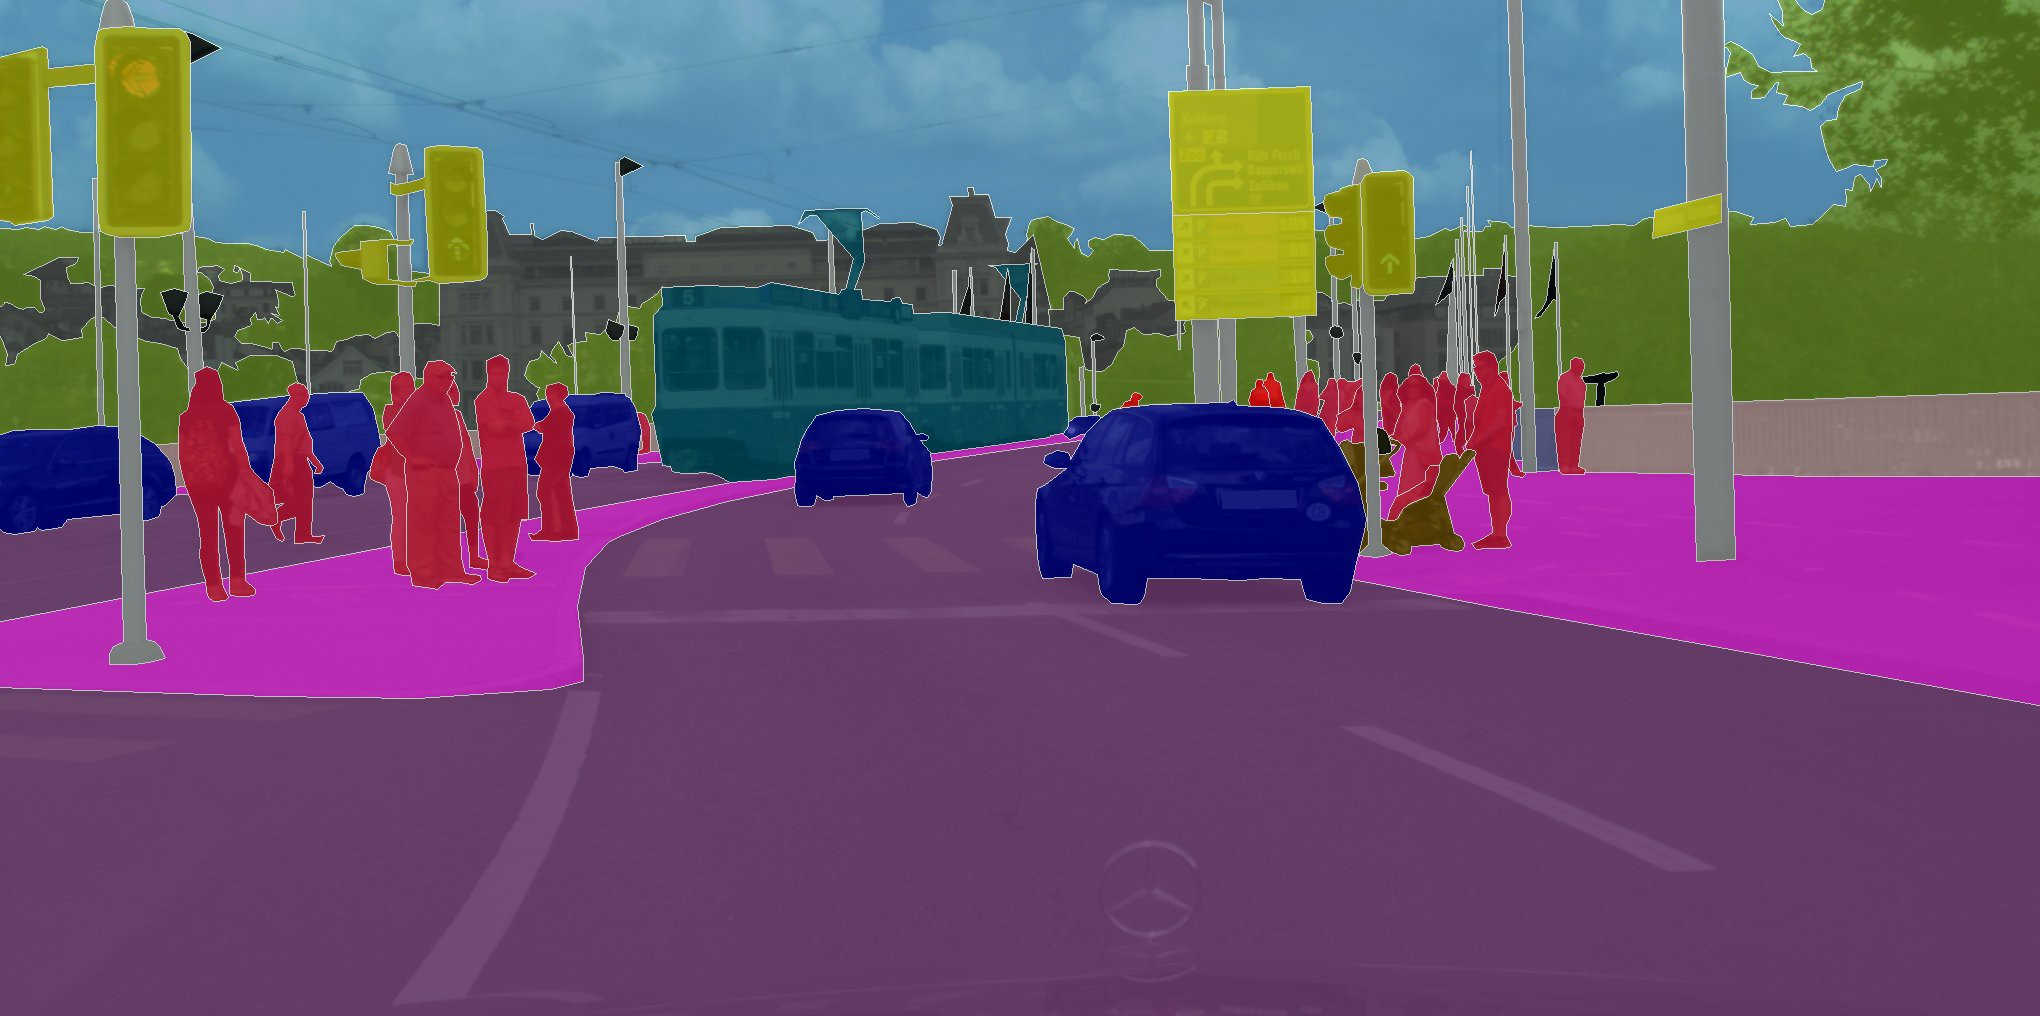
\includegraphics[width=\textwidth]{fig/semantic.jpeg}
% using a YouTube video



\end{columns}



\end{frame}

\subsection{Problem statement}
\begin{frame}{Problem statement}

Get the accurate neural network for semantic segmentation for DuckieTown,

\end{frame}



\subsection{Environment description}
\begin{frame}{Environment description}
\begin{columns}
\column{.6\textwidth}
\begin{itemize}
    \item Duckietown enviroment
    \item LGSVL Simulator
    \item ROS2
\end{itemize}

\column{.4\textwidth}
    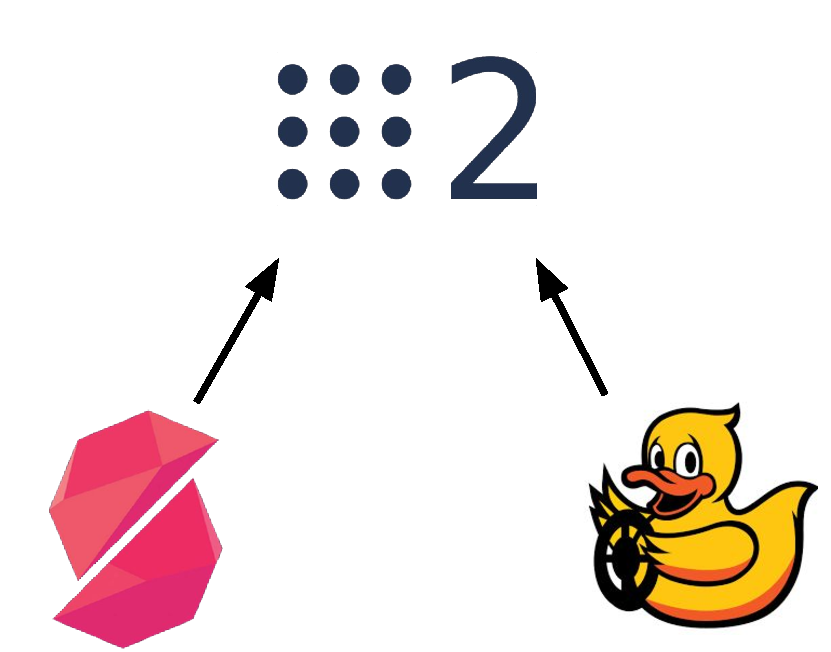
\includegraphics[width=0.75\textwidth]{fig/SS_AI.pdf}
\end{columns}

\end{frame}

\subsection{Significance of Research }
\begin{frame}{Significance of Research }
    \begin{itemize}
        \item Hands-on Deep Learning research
        \item Algorithms and techniques that are actually used in self-driving vehicles
        \item Possible contribution to ROS2 platform, which is currently under heavy-development
    \end{itemize}
\end{frame}

\section{Proposed solution}
    \subsection{To do}
    \begin{frame}{Proposed solution}

    \pause

    \begin{columns}

    \column{.4\textwidth}
        
\includegraphics[width=\textwidth]{fig/meme.jpeg}\pause

    \column{.6\textwidth}

    \begin{itemize}
        \item Hack the simulator to change the textures\pause
        \item Get the training data\pause
        \item Train the network\pause
        \item ?????\pause
        \item PROFIT!!!\pause
    \end{itemize}
    \end{columns}
    \end{frame}

    \subsection{Possible SW architecture}
    \begin{frame}{Possible SW architecture}
    % PIPELINE DIAGRAMS
    Sw part
    \end{frame}


\section{Conclusion}
\begin{frame}{Conclusion}
    \Huge \center Make DuckieTown great again!
    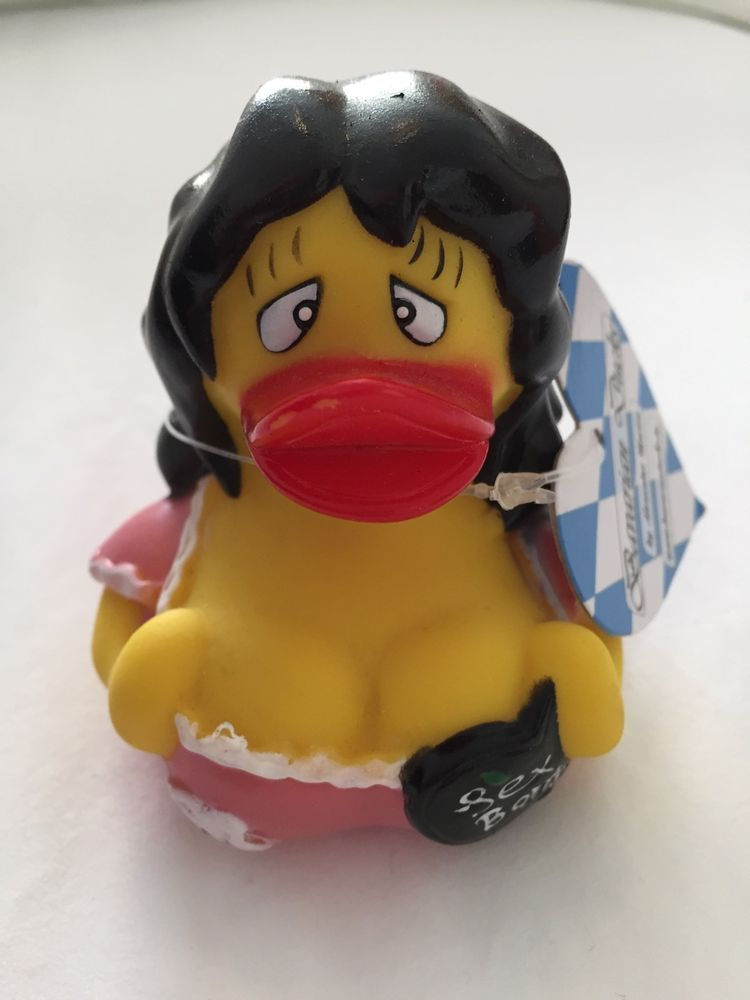
\includegraphics[height=4cm]{fig/duckie.jpg}
\end{frame}
\end{document}
